\section{Design af spoler}\label{sec:sec_spole_design}

\subsection{Dimensionering af spoler}

Systemet består af 3 spoler. 1 stor spole til at vidergive et signal, og 2 mindre spoler med samme areal til at opfange et signal. Dimensioneringen afhænger af størrelserne på spolerne. Der er nogle fysiske pladskrav, som begrænser dimensioneringen. Som udgangspunkt, dimensioneres den store spole først, som skal sende et signal videre. (omformuler blot udkast..)

Figur her!!

\begin{figure}[h!]
	\centering
	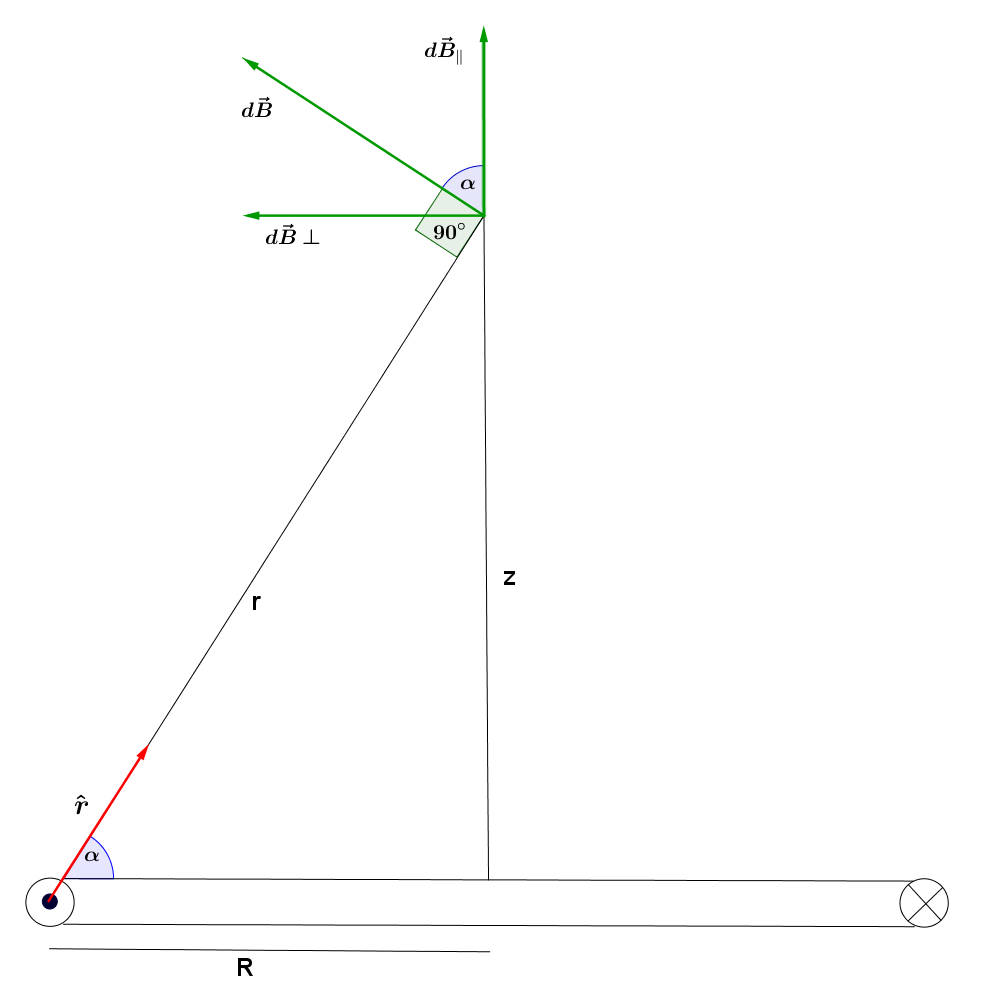
\includegraphics[width=.6\textwidth]{billeder/B_felt.png}
	\caption{test}
	\label{fig:BiotSavart1}
\end{figure}

 \begin{align}
 	&\vec{r'}=R(cos(\phi)\hat{i}+sin(\phi)\hat{j})
 \end{align}

\begin{align}
	&id\vec{s}=i\frac{d\vec{r'}}{d\phi}=i R d\phi (-sin(\phi)\hat{i}+cos(\phi)\hat{j})
\end{align}
Stedvektor:
\begin{align}
	&\vec{r_p}=z\hat{k}
\end{align}

relativ stedvektor
\begin{align}
	&\vec{r}=\vec{r_p}-\vec{r'}=-R cos(\phi)\hat{i}-sin(\phi)\hat{j}+z\hat{k}
\end{align}

Biot-savarts lov:
\begin{align}
	&d\vec{B}=\frac{\mu_0  i}{4\pi} \frac{d\vec{s} \times \hat{r}}{r^2}
\end{align}

\begin{align}
	&\hat{r}=\frac{\vec{r}}{r}
\end{align}

\begin{align}
	&r= \mid \vec{r} \mid = \sqrt{R^2+z^2}=\mid \vec{r_p}-\vec{r'} \mid
\end{align}



ganger igennem med ovenstående. (ligning?)

\begin{align}
	&d\vec{B}=\frac{\mu_0 i}{4\pi} \frac{d\vec{s} \times \vec{r}}{r^3}
\end{align}

	
\begin{align}
	&d\vec{s}\times(\vec{r_p}-\vec{r'})=R d\phi (-sin(\phi)\hat{i}+cos(\phi)\hat{j})\times (-R cos(\phi)\hat{i}-sin(\phi)\hat{j}+z\hat{k})
\end{align}	
Som yderligere kan reduceres ned til:

\begin{align}
	R \phi (z cos(\phi)\hat{i}+z sin(\phi)\hat{j}+R\hat{k})
\end{align}

\begin{align}
	&d\vec{B}=\frac{\mu_0 i}{4\pi} \frac{d\vec{s}\times (\vec{r_p}-\vec{r'})}{(\sqrt{R^2+z^2})^2}=\frac{\mu_0 i}{4\pi} \frac{R \phi (z cos(\phi)\hat{i}+z sin(\phi)\hat{j}+R\hat{k})}{(R^2+z^2)^\frac{3}{2}}
\end{align}


Ud fra dette, kan x og y komposanterne af B feltet sættes til = 0. Dette bevises ud fra:
\begin{align}
	&\frac{\mu_0 R z}{4\pi} \int\limits_{0}^{2\pi}cos(\phi)d\phi = 0
\end{align}


\begin{align}
	&\frac{\mu_0 R z}{4\pi} \int\limits_{0}^{2\pi}sin(\phi)d\phi = 0
\end{align}

Herefter er der kun z komposanten tilbage:
\begin{align}
	&B=\frac{\mu_0 R z}{4\pi} \int\limits_{0}^{2\pi}d\phi
\end{align}

Og dermed et udtryk for B i en cirkel.... (ret tekst her samt alle andre steder ved udledning.):


\begin{align}
	&B=\frac{\mu_0 iR^2 2\pi}{2(R^2+z^2)^\frac{3}{2}}
\end{align}




Tekst omkring solenoid her samt figur.



\begin{align}
	&di=inz'
\end{align}

\begin{align}
	&n=\frac{N}{L}
\end{align}

\begin{align}
	&d\vec{B}=\frac{\mu_0 R^2}{2[(z-z')^2+R^2]^\frac{3}{2}}di = \frac{\mu_0 R^2 i n dz'}{2[(z-z')^2+R^2]^\frac{3}{2}}
\end{align}


B felt i et givet punkt P centreret ud fra z aksen, med funktion af z er dermed givet ved:
\begin{align}
	&B(z)=\frac{\mu_0 n R^2 i}{2}\int\limits_{0}^{2\pi}\frac{1}{2[(z-z')^2+R^2]^\frac{3}{2}}dz'
\end{align}

\begin{align}
	&B(z)=\frac{\mu_0 n i}{2}\bigg[\frac{\frac{L}{2}-z}{\sqrt{(\frac{z-L}{2})^2+R^2}}+\frac{\frac{L}{2}+z}{\sqrt{(\frac{z+L}{2})^2+R^2}}\bigg]
\end{align}

\subsection{3D design/fysisk design af spolehus}
\begin{itemize}
	\item Inventor
	\item PnP system
	\item Huller til vindingsmaskine
	\item Clamp
\end{itemize}
Spolerne er designet således at når den store spole er i nul (i midten) overlapper den de mindre spoler så de er dækket præcist 50\percent. Når den store spole så er i sin fulde udslagsvinkel er hhv. den ene mindre spole dækket helt, hvor den anden slet ikke er dækket. \\

Illustration af forklaring her...
